% Benchmark Calibration Table
% !TEX TS-program = pdflatex
% !TEX options = -shell-escape -synctex=1 -interaction=nonstopmode -file-line-error "%DOC%"

\documentclass[margin=10pt, convert={outname=../images/distributedDiagram}]{standalone}    
\usepackage{pgfplots, pgf, natbib, textpos,ragged2e, colortbl, cancel, array, pgfplotstable, amsmath} 

\usetikzlibrary{calc, positioning, backgrounds, decorations.markings, external, arrows.meta, arrows, shapes, snakes, fit}
\usetikzlibrary{shapes,snakes}
\pgfplotsset{tick label style={font=\small}, label style={font=\small}, legend style={font=\small}, compat= newest}

\definecolor{UBCblue}{RGB}{12, 35, 68} 
\definecolor{UBClblue}{RGB}{0, 85, 183}
\definecolor{UBCgreen}{RGB}{88, 162, 41} 
\definecolor{UBCred}{RGB}{203, 29, 56}
\definecolor{UBCgrey}{RGB}{116, 145, 163}


\begin{document} 
	%<*tikzPic>
	
	\pgfplotsset{scale only axis, width=0.85\textwidth, height=0.5\textwidth}
	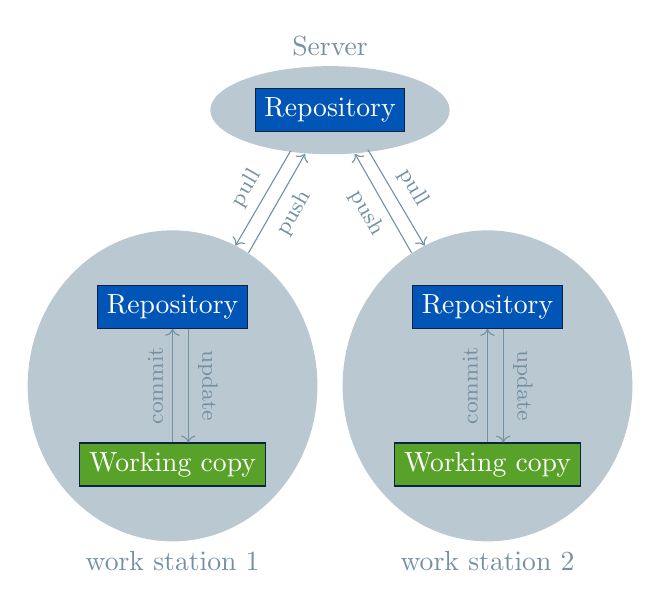
\begin{tikzpicture}[]
		
		% Server
		\node[shape=rectangle, draw=UBCblue, fill=UBClblue] (server) at (0,2.5) {\color{white}Repository};
		\begin{scope}[on background layer]
			\node[fit=(server), ellipse, fill=UBCgrey, opacity=0.5] (s1) {};
		\end{scope}
		\node[draw=none,fill=none, above = 0cm of s1] (a) {\color{UBCgrey}Server};
		% PC1
		\node[shape=rectangle, draw=UBCblue, fill=UBClblue] (pc1r) at (-2,0) {\color{white}Repository};
		\node[shape=rectangle, draw=UBCblue, fill=UBCgreen] (pc1) at (-2,-2) {\color{white}Working copy};
		\path[UBCgrey, ->] (pc1) edge node[midway, above, sloped] {\footnotesize commit} (pc1r);
		\path[UBCgrey, ->] ([xshift=2mm]pc1r.south) edge node[midway, above, sloped] {\footnotesize update} ([xshift=2mm]pc1.north);
		\begin{scope}[on background layer]
			\node[fit=(pc1r)(pc1), ellipse, fill=UBCgrey, opacity=0.5] (pc1a) {};
		\end{scope}
		\node[draw=none,fill=none, below = 0cm of pc1a] (b) {\color{UBCgrey}work station 1};

		% PC2
		\node[shape=rectangle, draw=UBCblue, fill=UBClblue] (pc2r) at (2,0) {\color{white}Repository};
		\node[shape=rectangle, draw=UBCblue, fill=UBCgreen] (pc2) at (2,-2) {\color{white}Working copy};
		\path[UBCgrey, ->] (pc2) edge node[midway, above, sloped] {\footnotesize commit} (pc2r);
		\path[UBCgrey, ->] ([xshift=2mm]pc2r.south) edge node[midway, above, sloped] {\footnotesize update} ([xshift=2mm]pc2.north);
		\begin{scope}[on background layer]
			\node[fit=(pc2r)(pc2), ellipse, fill=UBCgrey, opacity=0.5] (pc2a) {};
		\end{scope}
		\node[draw=none,fill=none, below = 0cm of pc2a] {\color{UBCgrey}work station 2};
		
		% connectors
		\path[UBCgrey, ->] (pc1a) edge node[midway, below, sloped] {\footnotesize push} (s1);
		\path[UBCgrey, ->] (pc2a) edge node[midway, below, sloped] {\footnotesize push} (s1);
		\path[UBCgrey, ->] ([xshift=-5mm, yshift=0.5mm]s1.south) edge node[midway, above, sloped] {\footnotesize pull} ([xshift=8mm, yshift=-2mm] pc1a.north);
		\path[UBCgrey, ->] ([xshift=-6mm, yshift=-1mm]s1.south east) edge node[midway, above, sloped] {\footnotesize pull} ([xshift=-8mm, yshift=-2mm] pc2a.north);
	\end{tikzpicture}%
	%</tikzPic>
	
\end{document}
